\documentclass[pdftex,beamer,svgnames]{beamer}

%\tiny, \scriptsize, \footnotesize, \small, \normalsize, \large, \Large, \LARGE, \huge, \Huge.

\usepackage{graphicx}
\usepackage{pgf}
\usepackage{amsmath,amssymb,euscript}
\usepackage[latin1]{inputenc}
\usepackage[procnames]{listings}
\usepackage{verbatim}
\usepackage{color}
\usepackage{hyperref}
\setcounter{tocdepth}{2}
\usepackage{tikz}
\usepackage{subfig}

\definecolor{keywords}{named}{DarkOrange}
\definecolor{comments}{named}{Green}
\definecolor{string}{named}{FireBrick}
\definecolor{link}{named}{blue}

\hypersetup{
    bookmarks=true,         % show bookmarks bar?
    colorlinks=true,       % false: boxed links; true: colored links
    allcolors=.,
    citecolor=blue,        % color of links to bibliography
    urlcolor=blue,           % color of external links
    anchorcolor=blue,
    %linkcolor=white,          % color of internal links (change box color with linkbordercolor)
    %filecolor=blue,      % color of file links
}

\lstdefinestyle{lststyle}{
    language=python,
    %basicstyle=\ttfamily\scriptsize, 
    basicstyle=\ttfamily\tiny,
    keywordstyle=\color{blue},
    commentstyle=\color{gray},
    stringstyle=\color{comments},
    showstringspaces=false,
    identifierstyle=\color{black},
    procnamekeys={def,class},
    %otherkeywords={osmose_demo, run_osmose, read_osmose},
    %deletekeywords={install, packages, demo, data, dir, read, file, path},
    %frame=single,
    frame=shadowbox,
    frameround=ffff,
    backgroundcolor=\color{gray!10!},
    %fillcolor=\color{green}
    rulesepcolor=\color{black}
}

\lstset{style=lststyle}

%\AtBeginSection[]
%{
%    \begin{frame}<beamer>
%        \frametitle{Table of Contents}
%        \tableofcontents[current,hideallsubsections]
%    \end{frame}
%}
%
%\AtBeginSubsection[]
%{
%    \begin{frame}<beamer>
%        \frametitle{Table of Contents}
%                  \tableofcontents[sectionstyle=show/shaded,subsectionstyle=show/shaded/hide]
%    \end{frame}
%}

\titlegraphic
{
{\parbox[c]{1.2cm}{
\includegraphics[scale=0.15]{../templates/logos/logo_ird.png}}}
\hspace{2cm}
{\parbox[c]{1.5cm}{
\includegraphics[scale=0.2]{../templates/logos/logo-marbec.png}}}
}


\setbeamertemplate{caption}[numbered]
\usetheme{AnnArbor}
%\usetheme{Copenhagen}
\definecolor{RRR}{rgb}{0.702,0.2,0.2}
\definecolor{bleuclair}{rgb}{0.9,0.9,1}
\definecolor{grisbleu}{rgb}{0.85,0.85,1}
\definecolor{monbleu}{rgb}{0,0.4,0.6}
\definecolor{bleuclair}{rgb}{0.9,0.9,1}
\definecolor{autrebleu}{rgb}{0.15,0.5,0.65}
\definecolor{bleufond}{rgb}{0.59,0.66,0.81}
\definecolor{bleufondplus}{rgb}{0.21,0.29,0.47}
\definecolor{monrouge}{rgb}{1,0.16,0.14}

\setbeamercolor{section in head/foot}{fg=white, bg=black}
\setbeamercolor{subsection in head/foot}{fg=white, bg=blue}
\setbeamercolor{title in head/foot}{fg=white, bg=blue}
\setbeamercolor{author in head/foot}{fg=white, bg=black}
\setbeamercolor{date in head/foot}{fg=white, bg=black}
\setbeamercolor{block body}{fg=black, bg=blue!10}
\setbeamercolor{block title}{fg=white, bg=blue}
\setbeamercolor{block body alerted}{fg=black, bg=FireBrick!10}
\setbeamercolor{block title alerted}{fg=white, bg=FireBrick}
\setbeamercolor{frametitle}{fg=white, bg=blue}
\setbeamercolor{title}{fg=white,bg=blue}

%\setbeamercolor{structure}{fg=black, bg=gray}
%\setbeamercolor{palette primary}{bg=orange,fg=yellow}
%\setbeamercolor{normal text}{fg=black,bg=white}
%\setbeamercolor{palette quaternary}{fg=black,bg=grisbleu}
%\setbeamercolor{palette sidebar tertiary}{bg=orange,fg=brown}
%\setbeamercolor{author}{fg=red,bg=brown}
%\setbeamercolor{title in head/foot}{fg=red,bg=black}
%\setbeamercolor{author in head/foot}{fg=green,bg=blue}
%\setbeamercolor{quotation}{fg=red}
%\setbeamercolor{subitem}{fg=red}
%\setbeamercolor{item}{fg=green}
%\setbeamercolor{bibliography item}{bg=black,fg=brown}
%\setbeamercolor {bibliography entry author}{fg=cyan,bg=orange}
%\setbeamercolor {bibliography entry location}{fg=magenta,bg=orange}
%\setbeamercolor{bibliography entry note}{fg=purple}
%\setbeamercolor{font quotation}{bg=cyan,fg=cyan}
%\setbeamercolor{quotation}{bg=cyan,fg=cyan}
%\setbeamercolor{quote}{bg=cyan,fg=cyan}
%


\beamertemplatenavigationsymbolsempty

\title[Python training for beginners]{Python training for beginners}
\author[nicolas.barrier@ird.fr]{Nicolas Barrier}
\date[May 26, 27, 28, 2020]{May 26, 27, 28, 2020}
\institute[IRD]{IRD, UMR MARBEC}


\subtitle{Data types: string, arrays (numpy, scipy)}

%%
%% Julia definition (c) 2014 Jubobs
%%
\lstdefinelanguage{julia}%
{morekeywords={abstract,break,case,catch,const,continue,do,else,elseif,%
end,export,false,for,function,immutable,import,importall,if,in,%
macro,module,otherwise,quote,return,switch,true,try,type,typealias,%
using,while},%
sensitive=true,%
alsoother={$},%
morecomment=[l]\#,%
morecomment=[n]{\#=}{=\#},%
morestring=[s]{"}{"},%
morestring=[m]{'}{'},%
}[keywords,comments,strings]%


\begin{document}

\frame{\titlepage}

\begin{frame}[fragile]
\frametitle{String usage}
String objects are very common in Python. They are especially usefull when reading and writting text files.\\

    \vspace{1em}
    They are defined between simple quotes (\verb+'+) or double quotes (\verb+"+). 

    \vspace{1em}
    \begin{alertblock}{Caution!}
        Opening and closing quotes must be the same
    \end{alertblock}
\end{frame}
    
\begin{frame}[fragile]
    \frametitle{Special characters}
    Python contains a set of predefined characters, which are listed below (source: \href{https://docs.python.org/3/reference/lexical_analysis.html}{python.org})

    \vspace{0.5em}
    \begin{center}
    \begin{tabular}{cc}
        Character &  Definition\\
        \hline
        \hline
        \verb+\a+ & ASCII Bell (BEL)\\
        \verb+\b+ & ASCII Backspace (BS)\\
        \verb+\f+ & ASCII Formfeed (FF)\\
        \verb+\n+ & ASCII Linefeed (LF)\\
        \verb+\r+ & ASCII Carriage Return (CR)\\
        \verb+\t+ & ASCII Horizontal Tab (TAB)\\
        \verb+\v+ & ASCII Vertical Tab (VT)\\
    \end{tabular}
    \end{center}

    \vspace{1em}
    In order to escape these special characters, add \verb+r+ before the 1st quote:
    \begin{lstlisting}[basicstyle=\ttfamily\scriptsize]
str1 = 'this is \t'
str2 = r'this is \t'
    \end{lstlisting}

\end{frame}

    \begin{frame}[fragile]
        \frametitle{String manipulation}

        String objects have a lot of methods to manipulate them. 
        \vspace{1em}

        Since they are \emph{immutable}, these methods return new string objects, compared to list methods, which
        change the list content.

    \vspace{1em}
    A very powerfull feature is the use of regular expressions, which allows to match strings with given patterns (\href{https://docs.python.org/3/library/re.html}{re} library).

    \vspace{1em}
    To learn a bit more on string manipulation, open the \verb+string.py+ file in Spyder.
\end{frame}

\begin{frame}[fragile]
\frametitle{Arrays}

    The Python \verb+list+ and \verb+dict+ objects are not suitable to manage multi-dimensional arrays. 
    \vspace{1em}

    Instead, the \href{https://numpy.org/}{Numpy} (Numerical Python) library should be used. It allows to:
    \begin{itemize}
        \item{Create multi-dimensional arrays}
        \item{Access array attributes (shape, number of dimensions, data types)}
        \item{Manipulate arrays (changing shape, tiling)}
        \item{Manipulate missing values} 
        \item{Perform optimized numerical operations (pointwise or matrix) via broadcasting (no loops)}
    \end{itemize}

    To manipulate arrays, play with the \verb+arrays.py+ file.

\end{frame}

\begin{frame}[fragile]
    \frametitle{Loops on multi-dimensional arrays}
    Computer memory is inherently linear, i.e. multi-dimensional arrays are stored in memory as one-dimensional arrays. This can be done in two ways:
    \begin{itemize}
        \item{Row-major order: C/C++, Python}
        \item{Column-major order: Fortran, Matlab, R, Julia}
    \end{itemize}

    \vspace{-1em}
    \begin{figure}
        \subfloat[Row-major order]{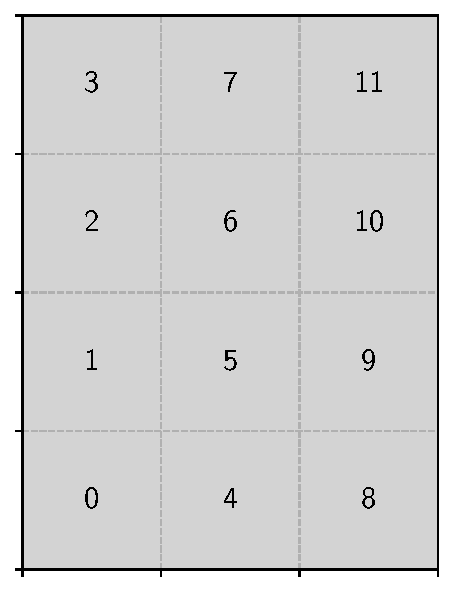
\includegraphics[scale=0.45]{figs/corder.pdf}}
        \qquad
        \subfloat[Column-major order]{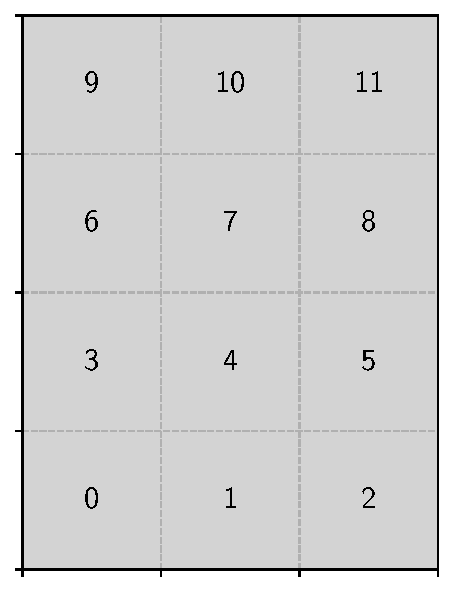
\includegraphics[scale=0.45]{figs/forder.pdf}}
    \end{figure}

\end{frame}

\begin{frame}[fragile]
    \frametitle{Loops on multi-dimensional arrays}
    Imbricated loops should be consistent with the memory ordering:

    \lstinputlisting[basicstyle=\ttfamily\scriptsize, caption={Row-order (Python)}]{scripts/loop.py}
    \lstinputlisting[basicstyle=\ttfamily\scriptsize,caption={Column-order (Julia)}, language=julia]{scripts/loop.jl}
    \vspace{1em}

    Sources: \href{https://en.wikipedia.org/wiki/Row-_and_column-major_order}{Wikipedia}, \href{https://eli.thegreenplace.net/2015/memory-layout-of-multi-dimensional-arrays/}{thegreenplace}

\end{frame}

\begin{frame}[fragile]
    \frametitle{Scientific Python}

    Although the Numpy library allows to do some operations, it is rather limited.
    Other mathematical functions are provided by the \href{https://www.scipy.org/}{Scipy} library. 

    \vspace{1em} 
    \emph{In an ideal world, NumPy would contain nothing but the array data type and the most basic operations: indexing, sorting, reshaping, basic elementwise functions, etc. All numerical code would reside in SciPy. [...] If you are doing scientific computing with Python, you should probably install both NumPy and SciPy. Most new features belong in SciPy rather than NumPy.} Source: \href{https://www.scipy.org/scipylib/faq.html#what-is-the-difference-between-numpy-and-scipy}{Scipy FAQ}

\end{frame}


\begin{frame}[fragile]
    \frametitle{Scientific Python: submodules}


    \begin{table}
        \centering
        \footnotesize
        \begin{tabular}{cc} 
            Description & Scipy submodule \\
            \hline
            \hline
            Special functions (mathematical physics) & \href{https://docs.scipy.org/doc/scipy/reference/tutorial/special.html}{scipy.special}\\
            Integration &\href{https://docs.scipy.org/doc/scipy/reference/tutorial/integrate.html}{scipy.integrate}\\
            Optimization &\href{https://docs.scipy.org/doc/scipy/reference/tutorial/optimize.html}{scipy.optimize}\\
            Interpolation &\href{https://docs.scipy.org/doc/scipy/reference/tutorial/optimize.html}{scipy.interpolate}\\
            Fourier Transforms &\href{https://docs.scipy.org/doc/scipy/reference/tutorial/fft.html}{scipy.fft}\\
            Signal Processing &\href{https://docs.scipy.org/doc/scipy/reference/tutorial/signal.html}{scipy.signal}\\
            Linear Algebra &\href{https://docs.scipy.org/doc/scipy/reference/tutorial/linalg.html}{scipy.linalg}\\
            Spatial data structures and algorithms & \href{https://docs.scipy.org/doc/scipy/reference/tutorial/spatial.html}{scipy.spatial}\\
            Statistics & \href{https://docs.scipy.org/doc/scipy/reference/tutorial/stats.html}{scipy.stats}\\
            Multidimensional image processing & \href{https://docs.scipy.org/doc/scipy/reference/tutorial/ndimage.html}{scipy.ndimage}\\
            File IO: \verb+.nc+, \verb+.mat+, \verb+.sav+ (IDL) &  \href{https://docs.scipy.org/doc/scipy/reference/tutorial/io.html}{scipy.io}\\
        \end{tabular}
        \caption{List of the Scipy submodules. Source: \href{https://www.scipy.org/}{scipy.org}}
    \end{table}

    \begin{block}{Sorry}
        Since you all are fluent in using Numpy, I leave it to you the exploration of Scipy...
    \end{block}

\end{frame}



\end{document}
